\section{Implementarea}

Implementarea \gls{wte} se bazează pe cod scris în limbajele Python, pentru nucleul simulatorului, ce implementează infrastructura și pe cod scris în limbajul C, pentru serverul \gls{netconf}, soluţia \gls{dvm} ce a fost dezvoltată anterior fiind adaptată pentru noua abordare. Codul este oferit cu sursă deschisă și poate fi găsit pe platforma GitHub~\cite{wte2017}. Paragrafele următoare vor prezenta detalii despre implementare, evidenţiind avantajele acestei abordări și motivele pentru care soluţia poate fi considerată un adevărat simulator de rețele de transport de date fără fir. 

\subsection{Fişierele de configurare}

\gls{wte} folosește fişiere de configurare, pentru a oferi o interfață simplă de configurare utilizatorilor. Există două fişiere scrise în limbajul \gls{json}, \textit{topology.json} și \textit{config.json}, primul pentru descrierea topologiei care va fi simulată și celălalt pentru a descrie caracteristicile configurabile ale simulatorului. Din aceeaşi categorie fac parte și modelele informaționale. Fişierele \gls{yang} asociate acestora sunt folosite de către simulator pentru a fi expuse de serverul \gls{netconf}.

Fişierul \gls{json} care descrie topologia are un format static, ce va fi prezentat în continuare. Acesta este ilustrat și în Figura \ref{fig:wte_topology_json}.

\begin{figure}[h]
	\centering
	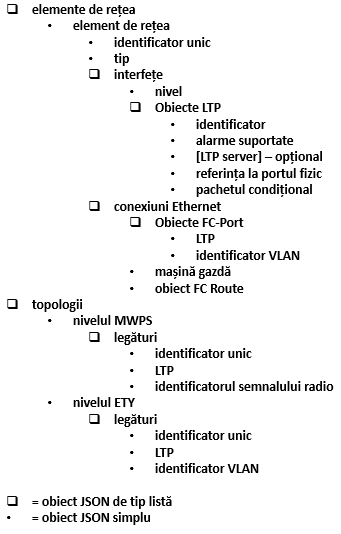
\includegraphics{wte_topology_json}
	\caption{Formatul fișierului JSON care descrie topologia rețelei simulată cu WTE.}
	\label{fig:wte_topology_json}
\end{figure}

Pentru descrierea topologiei unei rețele este suficient să cunoaştem dispozitivele și legăturile dintre acestea. Fiind rețele de transport de date fără fir, în cele mai simple cazuri, putem avea două tipuri de legături între echipamente: fără fir, sau legături Ethernet. Astfel, fişierul de topologie conţine două obiecte \gls{json} de tip listă: (i) \textbf{elemente de rețea} (\textit{network-elements}), ce descrie dispozitivele de rețea și (ii) \textbf{topologii} (\textit{topologies}), reprezentând legăturile dintre echipamente.

Fiecare element de rețea va avea mai multe detalii prezente în fişierul de topologie. Identificatorul unic reprezintă un nume unic ce va fi dat fiecărui dispozitiv de rețea, pentru a-l putea recunoaşte în topologia simulată. Tipul elementului se referă la soluţia ce va fi folosită pentru implementarea serverului \gls{netconf} ce va expune modelele informaționale dorite. În cazul alegerii \gls{dvm}, valoarea acestui element este \textit{OpenYuma}. Pentru cea de-a patra demonstraţie de concept \gls{onf}, o companie a folosit simulatorul \gls{wte} pentru dezvoltarea de aplicații \gls{sdn}, dar a preferat o soluție mai simplă, dar cu mai puţine capabilităţi pentru implementarea serverului \gls{netconf}, astfel că a folosit acest parametru pentru a informa nucleul simulatorului să folosească celălalt server. 

Elementul cel mai important al unui dispozitiv de rețea este reprezentat de obiectul \gls{json} de tip listă \textit{interfețe}, fiind responsabil pentru descrierea interfeţelor acelui dispozitiv. O interfață a unui echipament are ca echivalent un obiect \gls{ltp} din modelul informațional de bază. Obiectul \textit{nivel} din lista de interfețe reprezintă nivelul de transport asociat obiectului \gls{ltp}. Valorile pe care acesta le poate lua sunt descrise în modelul informațional de bază, în Capitolul \ref{ch:sdn_in_contextul_wt}: \gls{mwps}, \gls{mws}, \gls{etc}, \gls{ety} și \gls{eth}. Fiecare interfață prezintă câteva detalii de care simulatorul are nevoie: identificatorul obiectului \gls{ltp}, alarmele suportate (simulatorul are nevoie de această valoare, deoarece în modelul informațional pentru microunde, pe baza acestui atribut este definită lista alarmelor suportate și aceasta are un număr minim elemente; dacă nu este implementat acest număr minim, modelul \gls{yang} prezentat de serverul \gls{netconf} nu va fi valid), obiectul \gls{ltp} care reprezintă serverul pentru obiectul \gls{ltp} curent, dacă există (pentru reprezentarea relaţiilor de tip client-server dintre interfețe), referinţa la portul fizic și pachetul condiţional folosit de acest obiect \gls{ltp}.

Următorul obiect \gls{json} care face parte din fişierul de descriere a topologiei este tot un obiect de tip listă, \textit{conexiuni Ethernet}. Acestea reprezintă obiectele \gls{fc} definite în modelul informațional de bază. Practic, acestea exprimă conexiunile interne între interfeţele dispozitivului (de exemplu, traficul de pe o interfaţă radio R1 va fi dirijat către o interfață Ethernet E2). De aceea, obiectul \textit{conexiuni Ethernet} conţine două obiecte de tipul porturi \gls{fc}, care descriu exact această legătură internă. Obiectul \gls{json} \textit{mașină gazdă} care este prezent aici este folosit pentru simularea unei gazde care folosește această conexiune internă și este utilizat pentru generarea sau recepţionarea de trafic în cadrul simulatorului.

Obiectul \gls{json} \textit{topologii} descrie legăturile dintre dispozitivele de rețea. Există două niveluri de transport la care pot exista aceste conexiuni: \gls{mwps}, adică legăturile fără fir și \gls{ety}, reprezentând conexiunile Ethernet dintre echipamente. Fiecare legătură este reprezentată ca un obiect \gls{json} de tip listă, având doar două elemente, ce descriu cele două capete ale conexiunii, prin identificatorul unic al dispozitivului și identificatorul unic al interfeţei.

Cel de-al doilea fişier \gls{json} folosit de \gls{wte} este \textit{config.json}. Formatul acestuia poate fi observat în Figura \ref{fig:wte_config_json}.

\begin{figure}[h]
	\centering
	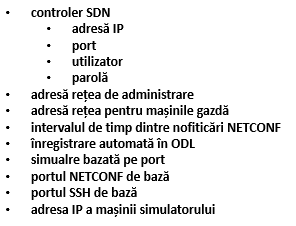
\includegraphics{wte_config_json}
	\caption{Formatul fişierului JSON de configurare a simulatorului WTE.}
	\label{fig:wte_config_json}
\end{figure}

Acesta conţine detaliile de conectare la echipamentul de control \gls{sdn}, în cazul în care se doreşte înregistrarea automată a dispozitivelor simulate la controler, constând în adresa IP, portul, numele de utilizator și parola folosite pentru autentificare. Următorul parametru descrie adresa rețelei de administrare care să fie folosită pentru alocarea adreselor IP pentru interfeţele de administrare ale echipamentelor simulate. În același mod se poate configura și plaja de adrese IP care să fie alocată maşinilor gazdă, folosite pentru generarea și recepţionarea traficului de date prin rețeaua simulată. 

Echipamentele simulate pot genera, la fel ca \gls{dvm}, notificări \gls{netconf} fictive. Intervalul de timp dintre două astfel de notificări este prezent în fişierul \gls{json} de configurare. Parametrul \textit{înregistrare automată în \gls{odl}} este folosit de către utilizator pentru a configura simulatorul să facă sau nu înregistrarea automată a dispozitivelor în echipamentul de control specificat prin detaliile de conectare anterioare. Metoda de înregistrare folosită este specifică echipamentului de control \gls{odl}, dar poate fi extinsă și pentru altele.

Următorii parametri sunt folosiţi în cazul în care utilizatorul nu doreşte adrese IP diferite pentru administrarea dispozitivelor simulate. Astfel, echipamentele vor putea fi accesate prin adresa IP a maşinii pe care rulează simulatorul, dar prin porturi diferite. De aceea, este nevoie ca utilizatorul să configureze portul de bază (portul de la care începe numărătoarea în momentul asignării porturilor pentru fiecare element de rețea simulat), pentru protocoalele \gls{netconf} și \gls{ssh}.

\subsection{Adaptarea DVM pentru WTE}

Folosirea \gls{dvm} fără o adaptare prealabilă la cerințele \gls{wte} nu ar fi fost posibilă. În primul rând, \gls{dvm} a fost transformat astfel încât să poată fi folosit într-un container \textit{docker}. Cerinţa pentru \gls{dvm} a fost să permită rularea mai multor instanţe, fiecare în containerul \textit{docker} asociat, însă având o configuraţie proprie la dispoziţie, în funcție de detaliile cuprinse în fişierul de descriere a topologiei.

Am decis astfel împărțirea atributelor prezente în modelele informaționale de bază și pentru microunde în două tipuri: de configurare și de stare. Dacă în versiunile anterioare, baza de stocare de date de execuţie se construia manual, pentru toate atributele, în codul C al serverului \gls{netconf}, această abordare nu ar mai fi fost posibilă, deoarece configurația era variată pentru diferitele dispozitive de rețea ce trebuie simulate. Am dezvoltat astfel o soluție automată care să construiască această bază de stocare de date de execuţie \gls{netconf}. În cazul atributelor de configurare, soluţia a fost folosirea unui fişier \gls{xml} care să le conţină, împreună cu conceptul bazei de stocare de date de iniţializare. Astfel, în momentul în care serverul \gls{netconf} porneşte, va încărca în baza de stocare de date de execuţie conţinutul acelui fişier de iniţializare. Dacă structura fişierului \gls{xml} este corectă, serverul \gls{netconf} va expune interfeţele și celelalte detalii oferite de atributele de configurare către echipamentul de control \gls{sdn}. Această soluție înseamnă, din punctul de vedere al nucleului \gls{wte}, construirea acelui fişier \gls{xml} astfel încât să aibă o structură corectă și să reflecte informaţiile din fişierul care descrie topologia ce trebuie simulată.

În cazul atributelor de stare, am renunţat la abordarea folosită anterior pentru \gls{dvm}, și anume împărțirea acestora în atribute de execuţie și de iniţializare, deoarece nu s-ar fi putut aplica într-o manieră automată. Soluția în acest caz a fost modificarea uneltei oferite de cadrul software \textit{OpenYuma}, care generează scheletul codului C din fişierul *.yang asociat modelului informațional. Acesta a fost alterat astfel încât să preia valoarea oricărui atribut de stare prezent în model dintr-un fişier \gls{xml} care conţine valorile acestor atribute. Astfel, din punctul de vedere al nucleului \gls{wte}, acest lucru înseamnă construirea unui fişier \gls{xml} care să conţină atributele de stare prezente în modelele \gls{yang} și valorile acestora.

Fiecare instanţă de server \gls{netconf} va avea la dispoziţie două fişiere \gls{xml}: unul care conţine valorile atributelor de configurare, reprezentând baza de stocare de date de iniţializare și celălalt cuprinzând atributele de stare, oferind utilizatorilor diferite valori implicite. Structura acestora este bazată pe modelele informaționale de bază și pentru microunde și este generată automat. Detalii despre această generare vor fi oferite în secţiunea următoare, în contextul prezentării nucleului \gls{wte}.

Mecanismul de generare a notificărilor \gls{netconf} fictive a fost îmbunătăţit în această versiune și este prezentat în Figura \ref{fig:wte_notif_generation}. 

\begin{figure}[h]
	\centering
	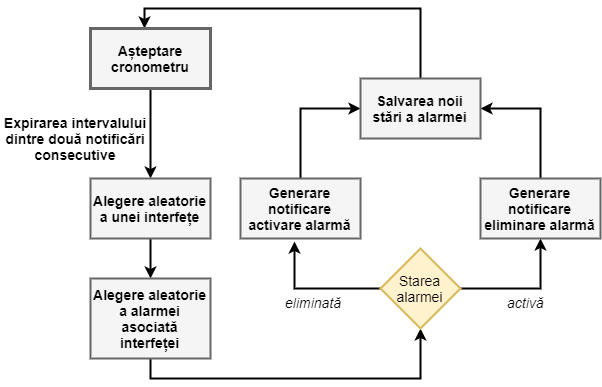
\includegraphics[width=1\textwidth]{wte_notif_generation}
	\caption{Organigrama mecanismului de generare a notificărilor NETCONF fictive al WTE.}
	\label{fig:wte_notif_generation}
\end{figure}

Până acum, generarea acestora se baza pe intervalul dintre două notificări consecutive definit în fişierul de configurare al \gls{dvm} și pe detaliile notificării ce se preluau din același loc. Acum, abordarea este diferită. În cazul notificărilor de tip \textit{valoarea atributului s-a schimbat - attributeValueChanged}, am modificat unealta care generează automat scheletul de cod C asociat serverului \gls{netconf}, astfel încât fiecare funcție cu apel invers asociată unui atribut configurabil va invoca funcţia ce trimite această notificare, conţinând valorile reale de care este nevoie: obiectul căruia i s-a schimbat valoare și noua valoare a acestuia. În acest mod, notificările de schimbare a valorii unui atribut nu mai sunt fictive, ci vor fi recepţionate de clienţii \gls{netconf} care s-au abonat la primirea acestora, chiar în momentul în care valoarea se schimbă. În cazul notificărilor de tip \textit{problemă - problemNotification}, sau alarmele pe care le generează dispozitivele de rețea, a fost păstrat principiul declanşării acestora în mod fictiv. Prin natura modelului informațional pentru microunde, fiecare interfață are asociată o listă de probleme pe care le poate avea și este definit și un număr minim de elemente pe care această listă să le aibă. \gls{wte} profită de acest aspect, implementând următorul mecanism de generare a alarmelor fictive: pentru fiecare problemă se retine starea acesteia: \textit{activă} sau \textit{eliminată}. Când intervalul dintre două notificări fictive consecutive s-a scurs, simulatorul se va pregăti să trimită o nouă notificare, astfel: se va alege în mod aleator o interfață a dispozitivului, iar din lista de probleme asociată interfeţei se va alege, din nou în mod aleator, o alarmă. În cazul în care starea acesteia este \textit{activă}, se trimite o notificare care conţine eliminarea acestei alarme și se schimbă starea asociată acestei probleme în \textit{eliminată}. Dacă starea acesteia era \textit{eliminată}, se va trimite o notificare care conţine activarea acestei probleme și starea ei va fi schimbată în \textit{activă}. Acest mecanism oferă dezvoltatorilor de aplicații \gls{sdn} un oarecare realism al simulatorului, alarmele fiind generate aleatoriu și, în cazul în care o alarmă era deja prezentă în echipamentul de control, există și posibilitatea ca această problemă să fie eliminată acum.

\subsection{Nucleul simulatorului WTE}



\subsection{Reprezentarea interfeţelor unui dispozitiv de rețea}

\subsection{Legăturile dintre interfeţele elementelor de rețea}

\subsection{Linia de comandă}

\subsection{Generarea traficului de date}